\documentclass[twoside]{book}

% Packages required by doxygen
\usepackage{fixltx2e}
\usepackage{calc}
\usepackage{doxygen}
\usepackage[export]{adjustbox} % also loads graphicx
\usepackage{graphicx}
\usepackage[utf8]{inputenc}
\usepackage{makeidx}
\usepackage{multicol}
\usepackage{multirow}
\PassOptionsToPackage{warn}{textcomp}
\usepackage{textcomp}
\usepackage[nointegrals]{wasysym}
\usepackage[table]{xcolor}

% Font selection
\usepackage[T1]{fontenc}
\usepackage[scaled=.90]{helvet}
\usepackage{courier}
\usepackage{amssymb}
\usepackage{sectsty}
\renewcommand{\familydefault}{\sfdefault}
\allsectionsfont{%
  \fontseries{bc}\selectfont%
  \color{darkgray}%
}
\renewcommand{\DoxyLabelFont}{%
  \fontseries{bc}\selectfont%
  \color{darkgray}%
}
\newcommand{\+}{\discretionary{\mbox{\scriptsize$\hookleftarrow$}}{}{}}

% Page & text layout
\usepackage{geometry}
\geometry{%
  a4paper,%
  top=2.5cm,%
  bottom=2.5cm,%
  left=2.5cm,%
  right=2.5cm%
}
\tolerance=750
\hfuzz=15pt
\hbadness=750
\setlength{\emergencystretch}{15pt}
\setlength{\parindent}{0cm}
\setlength{\parskip}{0.2cm}
\makeatletter
\renewcommand{\paragraph}{%
  \@startsection{paragraph}{4}{0ex}{-1.0ex}{1.0ex}{%
    \normalfont\normalsize\bfseries\SS@parafont%
  }%
}
\renewcommand{\subparagraph}{%
  \@startsection{subparagraph}{5}{0ex}{-1.0ex}{1.0ex}{%
    \normalfont\normalsize\bfseries\SS@subparafont%
  }%
}
\makeatother

% Headers & footers
\usepackage{fancyhdr}
\pagestyle{fancyplain}
\fancyhead[LE]{\fancyplain{}{\bfseries\thepage}}
\fancyhead[CE]{\fancyplain{}{}}
\fancyhead[RE]{\fancyplain{}{\bfseries\leftmark}}
\fancyhead[LO]{\fancyplain{}{\bfseries\rightmark}}
\fancyhead[CO]{\fancyplain{}{}}
\fancyhead[RO]{\fancyplain{}{\bfseries\thepage}}
\fancyfoot[LE]{\fancyplain{}{}}
\fancyfoot[CE]{\fancyplain{}{}}
\fancyfoot[RE]{\fancyplain{}{\bfseries\scriptsize Generated on Thu Feb 5 2015 16\+:40\+:35 for Kanban Board by Doxygen }}
\fancyfoot[LO]{\fancyplain{}{\bfseries\scriptsize Generated on Thu Feb 5 2015 16\+:40\+:35 for Kanban Board by Doxygen }}
\fancyfoot[CO]{\fancyplain{}{}}
\fancyfoot[RO]{\fancyplain{}{}}
\renewcommand{\footrulewidth}{0.4pt}
\renewcommand{\chaptermark}[1]{%
  \markboth{#1}{}%
}
\renewcommand{\sectionmark}[1]{%
  \markright{\thesection\ #1}%
}

% Indices & bibliography
\usepackage{natbib}
\usepackage[titles]{tocloft}
\setcounter{tocdepth}{3}
\setcounter{secnumdepth}{5}
\makeindex

% Hyperlinks (required, but should be loaded last)
\usepackage{ifpdf}
\ifpdf
  \usepackage[pdftex,pagebackref=true]{hyperref}
\else
  \usepackage[ps2pdf,pagebackref=true]{hyperref}
\fi
\hypersetup{%
  colorlinks=true,%
  linkcolor=blue,%
  citecolor=blue,%
  unicode%
}

% Custom commands
\newcommand{\clearemptydoublepage}{%
  \newpage{\pagestyle{empty}\cleardoublepage}%
}


%===== C O N T E N T S =====

\begin{document}

% Titlepage & ToC
\hypersetup{pageanchor=false,
             bookmarks=true,
             bookmarksnumbered=true,
             pdfencoding=unicode
            }
\pagenumbering{roman}
\begin{titlepage}
\vspace*{7cm}
\begin{center}%
{\Large Kanban Board \\[1ex]\large 1 }\\
\vspace*{1cm}
{\large Generated by Doxygen 1.8.9.1}\\
\vspace*{0.5cm}
{\small Thu Feb 5 2015 16:40:35}\\
\end{center}
\end{titlepage}
\clearemptydoublepage
\tableofcontents
\clearemptydoublepage
\pagenumbering{arabic}
\hypersetup{pageanchor=true}

%--- Begin generated contents ---
\chapter{Namespace Index}
\section{Packages}
Here are the packages with brief descriptions (if available)\+:\begin{DoxyCompactList}
\item\contentsline{section}{\hyperlink{namespace_helper_classes}{Helper\+Classes} }{\pageref{namespace_helper_classes}}{}
\item\contentsline{section}{\hyperlink{namespace_kanban_board}{Kanban\+Board} }{\pageref{namespace_kanban_board}}{}
\item\contentsline{section}{\hyperlink{namespace_kanban_board_1_1_model}{Kanban\+Board.\+Model} }{\pageref{namespace_kanban_board_1_1_model}}{}
\item\contentsline{section}{\hyperlink{namespace_kanban_board_1_1_persistence}{Kanban\+Board.\+Persistence} }{\pageref{namespace_kanban_board_1_1_persistence}}{}
\item\contentsline{section}{\hyperlink{namespace_kanban_board_1_1_view_model}{Kanban\+Board.\+View\+Model} }{\pageref{namespace_kanban_board_1_1_view_model}}{}
\end{DoxyCompactList}

\chapter{Hierarchical Index}
\section{Class Hierarchy}
This inheritance list is sorted roughly, but not completely, alphabetically\+:\begin{DoxyCompactList}
\item \contentsline{section}{Kanban\+Board.\+View\+Model.\+Category\+View\+Model}{\pageref{class_kanban_board_1_1_view_model_1_1_category_view_model}}{}
\item \contentsline{section}{Kanban\+Board.\+View\+Model.\+Employee\+View\+Model}{\pageref{class_kanban_board_1_1_view_model_1_1_employee_view_model}}{}
\item I\+Command\begin{DoxyCompactList}
\item \contentsline{section}{Helper\+Classes.\+Relay\+Command}{\pageref{class_helper_classes_1_1_relay_command}}{}
\end{DoxyCompactList}
\item I\+Drop\+Target\begin{DoxyCompactList}
\item \contentsline{section}{Kanban\+Board.\+View\+Model.\+Main\+View\+Model}{\pageref{class_kanban_board_1_1_view_model_1_1_main_view_model}}{}
\end{DoxyCompactList}
\item I\+Notify\+Property\+Changed\begin{DoxyCompactList}
\item \contentsline{section}{Kanban\+Board.\+View\+Model.\+Main\+View\+Model}{\pageref{class_kanban_board_1_1_view_model_1_1_main_view_model}}{}
\end{DoxyCompactList}
\item \contentsline{section}{Kanban\+Board.\+Persistence.\+I\+Persistence}{\pageref{interface_kanban_board_1_1_persistence_1_1_i_persistence}}{}
\begin{DoxyCompactList}
\item \contentsline{section}{Kanban\+Board.\+Persistence.\+Persistence\+Handler.\+Json\+Persistence}{\pageref{class_kanban_board_1_1_persistence_1_1_persistence_handler_1_1_json_persistence}}{}
\item \contentsline{section}{Kanban\+Board.\+Persistence.\+Persistence\+Handler.\+Xml\+Persistence}{\pageref{class_kanban_board_1_1_persistence_1_1_persistence_handler_1_1_xml_persistence}}{}
\end{DoxyCompactList}
\item \contentsline{section}{Kanban\+Board.\+View\+Model.\+Manipulate\+Post\+It\+View\+Model}{\pageref{class_kanban_board_1_1_view_model_1_1_manipulate_post_it_view_model}}{}
\item \contentsline{section}{Kanban\+Board.\+Persistence.\+Persistence\+Handler}{\pageref{class_kanban_board_1_1_persistence_1_1_persistence_handler}}{}
\item \contentsline{section}{Kanban\+Board.\+Model.\+Person\+Model}{\pageref{class_kanban_board_1_1_model_1_1_person_model}}{}
\begin{DoxyCompactList}
\item \contentsline{section}{Kanban\+Board.\+Model.\+Employee\+Model}{\pageref{class_kanban_board_1_1_model_1_1_employee_model}}{}
\end{DoxyCompactList}
\item \contentsline{section}{Kanban\+Board.\+Model.\+Post\+It\+Model}{\pageref{class_kanban_board_1_1_model_1_1_post_it_model}}{}
\item \contentsline{section}{Kanban\+Board.\+Model.\+Settings\+Model}{\pageref{class_kanban_board_1_1_model_1_1_settings_model}}{}
\end{DoxyCompactList}

\chapter{Class Index}
\section{Class List}
Here are the classes, structs, unions and interfaces with brief descriptions\+:\begin{DoxyCompactList}
\item\contentsline{section}{\hyperlink{class_kanban_board_1_1_view_model_1_1_category_view_model}{Kanban\+Board.\+View\+Model.\+Category\+View\+Model} }{\pageref{class_kanban_board_1_1_view_model_1_1_category_view_model}}{}
\item\contentsline{section}{\hyperlink{interface_kanban_board_1_1_persistence_1_1_i_persistence}{Kanban\+Board.\+Persistence.\+I\+Persistence} }{\pageref{interface_kanban_board_1_1_persistence_1_1_i_persistence}}{}
\item\contentsline{section}{\hyperlink{class_kanban_board_1_1_persistence_1_1_persistence_handler_1_1_json_persistence}{Kanban\+Board.\+Persistence.\+Persistence\+Handler.\+Json\+Persistence} \\*This class will use the newtonsoft json package to serialize and deserialize }{\pageref{class_kanban_board_1_1_persistence_1_1_persistence_handler_1_1_json_persistence}}{}
\item\contentsline{section}{\hyperlink{class_kanban_board_1_1_view_model_1_1_main_view_model}{Kanban\+Board.\+View\+Model.\+Main\+View\+Model} }{\pageref{class_kanban_board_1_1_view_model_1_1_main_view_model}}{}
\item\contentsline{section}{\hyperlink{class_kanban_board_1_1_view_model_1_1_manipulate_post_it_view_model}{Kanban\+Board.\+View\+Model.\+Manipulate\+Post\+It\+View\+Model} }{\pageref{class_kanban_board_1_1_view_model_1_1_manipulate_post_it_view_model}}{}
\item\contentsline{section}{\hyperlink{class_kanban_board_1_1_persistence_1_1_persistence_handler}{Kanban\+Board.\+Persistence.\+Persistence\+Handler} \\*Handles the different types of persistence }{\pageref{class_kanban_board_1_1_persistence_1_1_persistence_handler}}{}
\item\contentsline{section}{\hyperlink{class_kanban_board_1_1_model_1_1_person_model}{Kanban\+Board.\+Model.\+Person\+Model} }{\pageref{class_kanban_board_1_1_model_1_1_person_model}}{}
\item\contentsline{section}{\hyperlink{class_kanban_board_1_1_model_1_1_post_it_model}{Kanban\+Board.\+Model.\+Post\+It\+Model} }{\pageref{class_kanban_board_1_1_model_1_1_post_it_model}}{}
\item\contentsline{section}{\hyperlink{class_helper_classes_1_1_relay_command}{Helper\+Classes.\+Relay\+Command} \\*A command whose sole purpose is to relay its functionality to other objects by invoking delegates. The default return value for the Can\+Execute method is \textquotesingle{}true\textquotesingle{}. \hyperlink{class_helper_classes_1_1_relay_command_a14af980403ef90c4ee57f1395988fa8e}{Raise\+Can\+Execute\+Changed} needs to be called whenever \hyperlink{class_helper_classes_1_1_relay_command_a1e2d080059a2f0f7cd455af612d77bbe}{Can\+Execute} is expected to return a different value. }{\pageref{class_helper_classes_1_1_relay_command}}{}
\end{DoxyCompactList}

\chapter{Namespace Documentation}
\hypertarget{namespace_helper_classes}{}\section{Package Helper\+Classes}
\label{namespace_helper_classes}\index{Helper\+Classes@{Helper\+Classes}}
\subsection*{Classes}
\begin{DoxyCompactItemize}
\item 
class \hyperlink{class_helper_classes_1_1_relay_command}{Relay\+Command}
\begin{DoxyCompactList}\small\item\em A command whose sole purpose is to relay its functionality to other objects by invoking delegates. The default return value for the Can\+Execute method is \textquotesingle{}true\textquotesingle{}. \hyperlink{class_helper_classes_1_1_relay_command_a14af980403ef90c4ee57f1395988fa8e}{Raise\+Can\+Execute\+Changed} needs to be called whenever \hyperlink{class_helper_classes_1_1_relay_command_a1e2d080059a2f0f7cd455af612d77bbe}{Can\+Execute} is expected to return a different value. \end{DoxyCompactList}\end{DoxyCompactItemize}

\hypertarget{namespace_kanban_board}{}\section{Package Kanban\+Board}
\label{namespace_kanban_board}\index{Kanban\+Board@{Kanban\+Board}}
\subsection*{Namespaces}
\begin{DoxyCompactItemize}
\item 
package \hyperlink{namespace_kanban_board_1_1_model}{Model}
\item 
package \hyperlink{namespace_kanban_board_1_1_persistence}{Persistence}
\item 
package \hyperlink{namespace_kanban_board_1_1_view_model}{View\+Model}
\end{DoxyCompactItemize}

\hypertarget{namespace_kanban_board_1_1_model}{}\section{Package Kanban\+Board.\+Model}
\label{namespace_kanban_board_1_1_model}\index{Kanban\+Board.\+Model@{Kanban\+Board.\+Model}}
\subsection*{Classes}
\begin{DoxyCompactItemize}
\item 
class \hyperlink{class_kanban_board_1_1_model_1_1_employee_model}{Employee\+Model}
\item 
class \hyperlink{class_kanban_board_1_1_model_1_1_person_model}{Person\+Model}
\item 
class \hyperlink{class_kanban_board_1_1_model_1_1_post_it_model}{Post\+It\+Model}
\item 
class \hyperlink{class_kanban_board_1_1_model_1_1_settings_model}{Settings\+Model}
\end{DoxyCompactItemize}

\hypertarget{namespace_kanban_board_1_1_persistence}{}\section{Package Kanban\+Board.\+Persistence}
\label{namespace_kanban_board_1_1_persistence}\index{Kanban\+Board.\+Persistence@{Kanban\+Board.\+Persistence}}
\subsection*{Classes}
\begin{DoxyCompactItemize}
\item 
interface \hyperlink{interface_kanban_board_1_1_persistence_1_1_i_persistence}{I\+Persistence}
\item 
class \hyperlink{class_kanban_board_1_1_persistence_1_1_persistence_handler}{Persistence\+Handler}
\begin{DoxyCompactList}\small\item\em Handles the different types of persistence \end{DoxyCompactList}\end{DoxyCompactItemize}

\hypertarget{namespace_kanban_board_1_1_view_model}{}\section{Package Kanban\+Board.\+View\+Model}
\label{namespace_kanban_board_1_1_view_model}\index{Kanban\+Board.\+View\+Model@{Kanban\+Board.\+View\+Model}}
\subsection*{Classes}
\begin{DoxyCompactItemize}
\item 
class \hyperlink{class_kanban_board_1_1_view_model_1_1_category_view_model}{Category\+View\+Model}
\item 
class \hyperlink{class_kanban_board_1_1_view_model_1_1_main_view_model}{Main\+View\+Model}
\item 
class \hyperlink{class_kanban_board_1_1_view_model_1_1_manipulate_post_it_view_model}{Manipulate\+Post\+It\+View\+Model}
\end{DoxyCompactItemize}

\chapter{Class Documentation}
\hypertarget{class_kanban_board_1_1_view_model_1_1_category_view_model}{}\section{Kanban\+Board.\+View\+Model.\+Category\+View\+Model Class Reference}
\label{class_kanban_board_1_1_view_model_1_1_category_view_model}\index{Kanban\+Board.\+View\+Model.\+Category\+View\+Model@{Kanban\+Board.\+View\+Model.\+Category\+View\+Model}}


The documentation for this class was generated from the following file\+:\begin{DoxyCompactItemize}
\item 
d\+:/\+Dokumenter/\+Visual Studio 2013/\+Projects/2. Semester/\+Kanban\+Board/\+Kanban\+Board/\+View\+Model/Category\+View\+Model.\+cs\end{DoxyCompactItemize}

\hypertarget{interface_kanban_board_1_1_persistence_1_1_i_persistence}{}\section{Kanban\+Board.\+Persistence.\+I\+Persistence Interface Reference}
\label{interface_kanban_board_1_1_persistence_1_1_i_persistence}\index{Kanban\+Board.\+Persistence.\+I\+Persistence@{Kanban\+Board.\+Persistence.\+I\+Persistence}}
Inheritance diagram for Kanban\+Board.\+Persistence.\+I\+Persistence\+:\begin{figure}[H]
\begin{center}
\leavevmode
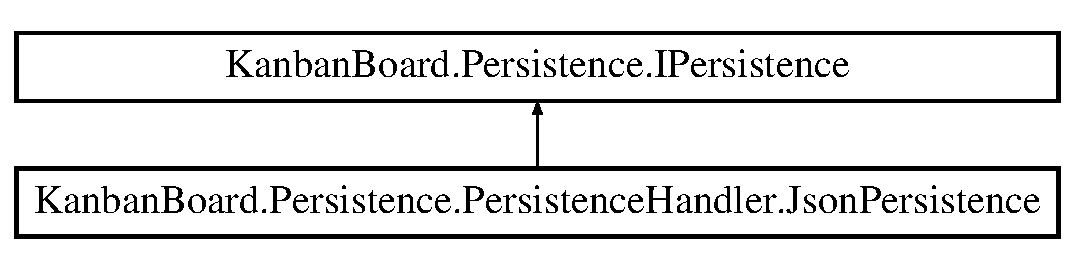
\includegraphics[height=1.477572cm]{interface_kanban_board_1_1_persistence_1_1_i_persistence}
\end{center}
\end{figure}


The documentation for this interface was generated from the following file\+:\begin{DoxyCompactItemize}
\item 
d\+:/\+Dokumenter/\+Visual Studio 2013/\+Projects/2. Semester/\+Kanban\+Board/\+Kanban\+Board/\+Persistence/I\+Persistence.\+cs\end{DoxyCompactItemize}

\hypertarget{class_kanban_board_1_1_persistence_1_1_persistence_handler_1_1_json_persistence}{}\section{Kanban\+Board.\+Persistence.\+Persistence\+Handler.\+Json\+Persistence Class Reference}
\label{class_kanban_board_1_1_persistence_1_1_persistence_handler_1_1_json_persistence}\index{Kanban\+Board.\+Persistence.\+Persistence\+Handler.\+Json\+Persistence@{Kanban\+Board.\+Persistence.\+Persistence\+Handler.\+Json\+Persistence}}


This class will use the newtonsoft json package to serialize and deserialize  


Inheritance diagram for Kanban\+Board.\+Persistence.\+Persistence\+Handler.\+Json\+Persistence\+:\begin{figure}[H]
\begin{center}
\leavevmode
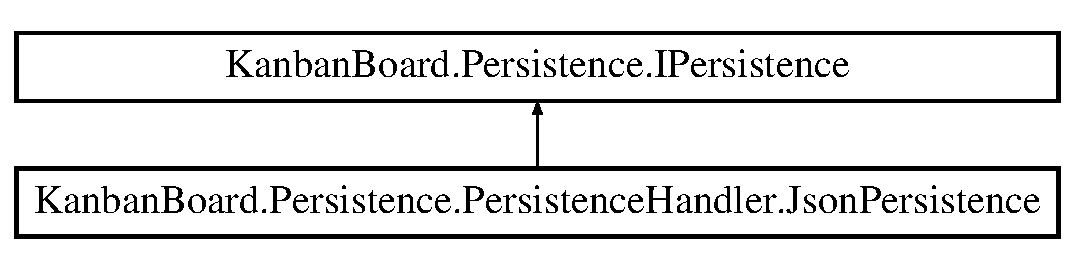
\includegraphics[height=2.000000cm]{class_kanban_board_1_1_persistence_1_1_persistence_handler_1_1_json_persistence}
\end{center}
\end{figure}
\subsection*{Public Member Functions}
\begin{DoxyCompactItemize}
\item 
void \hyperlink{class_kanban_board_1_1_persistence_1_1_persistence_handler_1_1_json_persistence_a925b52aa9fac036eaa854ab9f3be1e88}{Save} (Dictionary$<$ Enum\+Categories, \hyperlink{class_kanban_board_1_1_view_model_1_1_category_view_model}{Category\+View\+Model} $>$ information\+To\+Save, string file\+Name)
\begin{DoxyCompactList}\small\item\em Saves the post its in the categories. \end{DoxyCompactList}\item 
Dictionary$<$ Enum\+Categories, \hyperlink{class_kanban_board_1_1_view_model_1_1_category_view_model}{Category\+View\+Model} $>$ \hyperlink{class_kanban_board_1_1_persistence_1_1_persistence_handler_1_1_json_persistence_a03590c4676da93617e2b6738e22f5844}{Load} (string file\+Name)
\begin{DoxyCompactList}\small\item\em Loads the post its from a file \end{DoxyCompactList}\end{DoxyCompactItemize}


\subsection{Detailed Description}
This class will use the newtonsoft json package to serialize and deserialize 



\subsection{Member Function Documentation}
\hypertarget{class_kanban_board_1_1_persistence_1_1_persistence_handler_1_1_json_persistence_a03590c4676da93617e2b6738e22f5844}{}\index{Kanban\+Board\+::\+Persistence\+::\+Persistence\+Handler\+::\+Json\+Persistence@{Kanban\+Board\+::\+Persistence\+::\+Persistence\+Handler\+::\+Json\+Persistence}!Load@{Load}}
\index{Load@{Load}!Kanban\+Board\+::\+Persistence\+::\+Persistence\+Handler\+::\+Json\+Persistence@{Kanban\+Board\+::\+Persistence\+::\+Persistence\+Handler\+::\+Json\+Persistence}}
\subsubsection[{Load}]{\setlength{\rightskip}{0pt plus 5cm}Dictionary$<$Enum\+Categories, {\bf Category\+View\+Model}$>$ Kanban\+Board.\+Persistence.\+Persistence\+Handler.\+Json\+Persistence.\+Load (
\begin{DoxyParamCaption}
\item[{string}]{file\+Name}
\end{DoxyParamCaption}
)}\label{class_kanban_board_1_1_persistence_1_1_persistence_handler_1_1_json_persistence_a03590c4676da93617e2b6738e22f5844}


Loads the post its from a file 


\begin{DoxyParams}{Parameters}
{\em file\+Name} & The file to load from\\
\hline
\end{DoxyParams}
\begin{DoxyReturn}{Returns}
The post its that was loaded
\end{DoxyReturn}


Implements \hyperlink{interface_kanban_board_1_1_persistence_1_1_i_persistence}{Kanban\+Board.\+Persistence.\+I\+Persistence}.

\hypertarget{class_kanban_board_1_1_persistence_1_1_persistence_handler_1_1_json_persistence_a925b52aa9fac036eaa854ab9f3be1e88}{}\index{Kanban\+Board\+::\+Persistence\+::\+Persistence\+Handler\+::\+Json\+Persistence@{Kanban\+Board\+::\+Persistence\+::\+Persistence\+Handler\+::\+Json\+Persistence}!Save@{Save}}
\index{Save@{Save}!Kanban\+Board\+::\+Persistence\+::\+Persistence\+Handler\+::\+Json\+Persistence@{Kanban\+Board\+::\+Persistence\+::\+Persistence\+Handler\+::\+Json\+Persistence}}
\subsubsection[{Save}]{\setlength{\rightskip}{0pt plus 5cm}void Kanban\+Board.\+Persistence.\+Persistence\+Handler.\+Json\+Persistence.\+Save (
\begin{DoxyParamCaption}
\item[{Dictionary$<$ Enum\+Categories, {\bf Category\+View\+Model} $>$}]{information\+To\+Save, }
\item[{string}]{file\+Name}
\end{DoxyParamCaption}
)}\label{class_kanban_board_1_1_persistence_1_1_persistence_handler_1_1_json_persistence_a925b52aa9fac036eaa854ab9f3be1e88}


Saves the post its in the categories. 


\begin{DoxyParams}{Parameters}
{\em information\+To\+Save} & The post its that will be saved\\
\hline
{\em file\+Name} & The path to the file that will be saved to\\
\hline
\end{DoxyParams}


Implements \hyperlink{interface_kanban_board_1_1_persistence_1_1_i_persistence}{Kanban\+Board.\+Persistence.\+I\+Persistence}.



The documentation for this class was generated from the following file\+:\begin{DoxyCompactItemize}
\item 
d\+:/\+Dokumenter/\+Visual Studio 2013/\+Projects/2. Semester/\+Kanban\+Board/\+Kanban\+Board/\+Persistence/Persistence\+Handler.\+cs\end{DoxyCompactItemize}

\hypertarget{class_kanban_board_1_1_view_model_1_1_main_view_model}{}\section{Kanban\+Board.\+View\+Model.\+Main\+View\+Model Class Reference}
\label{class_kanban_board_1_1_view_model_1_1_main_view_model}\index{Kanban\+Board.\+View\+Model.\+Main\+View\+Model@{Kanban\+Board.\+View\+Model.\+Main\+View\+Model}}
Inheritance diagram for Kanban\+Board.\+View\+Model.\+Main\+View\+Model\+:\begin{figure}[H]
\begin{center}
\leavevmode
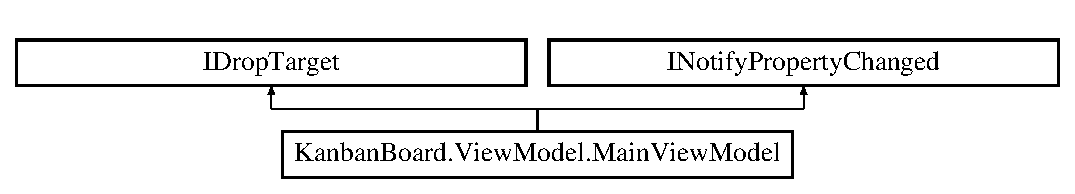
\includegraphics[height=2.000000cm]{class_kanban_board_1_1_view_model_1_1_main_view_model}
\end{center}
\end{figure}
\subsection*{Public Member Functions}
\begin{DoxyCompactItemize}
\item 
void \hyperlink{class_kanban_board_1_1_view_model_1_1_main_view_model_afeac47ff8c81ee187966b321dcd0adfd}{Drag\+Over} (I\+Drop\+Info drop\+Info)
\begin{DoxyCompactList}\small\item\em Updates the current drag state. Remarks\+: To allow a drop at the current drag position, the Gong\+Solutions.\+Wpf.\+Drag\+Drop.\+Drop\+Info.\+Effects property on drop\+Info should be set to a value other than System.\+Windows.\+Drag\+Drop\+Effects.\+None and Gong\+Solutions.\+Wpf.\+Drag\+Drop.\+Drop\+Info.\+Data should be set to a non-\/null value. \end{DoxyCompactList}\item 
void \hyperlink{class_kanban_board_1_1_view_model_1_1_main_view_model_a8a289987889845510435516f3699495c}{Drop} (I\+Drop\+Info drop\+Info)
\begin{DoxyCompactList}\small\item\em Performs a drop. And changes the colour of the posit it, according to the target. \end{DoxyCompactList}\end{DoxyCompactItemize}
\subsection*{Properties}
\begin{DoxyCompactItemize}
\item 
Observable\+Collection$<$ \hyperlink{class_kanban_board_1_1_model_1_1_post_it_model}{Post\+It\+Model} $>$ \hyperlink{class_kanban_board_1_1_view_model_1_1_main_view_model_a250c79012624be5145f7a08ce9fdd4d8}{List\+Of\+To\+Do}\hspace{0.3cm}{\ttfamily  \mbox{[}get, set\mbox{]}}
\begin{DoxyCompactList}\small\item\em Provides access to the List Of To do \end{DoxyCompactList}\item 
Observable\+Collection$<$ \hyperlink{class_kanban_board_1_1_model_1_1_post_it_model}{Post\+It\+Model} $>$ \hyperlink{class_kanban_board_1_1_view_model_1_1_main_view_model_ac28a6f8225d24e60ea7f1196cbf8d6a3}{List\+Of\+Work\+In\+Progress}\hspace{0.3cm}{\ttfamily  \mbox{[}get, set\mbox{]}}
\begin{DoxyCompactList}\small\item\em Provides access to the Lisf Of Work In Progress. \end{DoxyCompactList}\item 
Observable\+Collection$<$ \hyperlink{class_kanban_board_1_1_model_1_1_post_it_model}{Post\+It\+Model} $>$ \hyperlink{class_kanban_board_1_1_view_model_1_1_main_view_model_a6ecd7d9718b6e320441c5938dc1c01eb}{List\+Of\+Completed\+Work}\hspace{0.3cm}{\ttfamily  \mbox{[}get, set\mbox{]}}
\begin{DoxyCompactList}\small\item\em Provides access to the list of Completed Work. \end{DoxyCompactList}\item 
I\+Command \hyperlink{class_kanban_board_1_1_view_model_1_1_main_view_model_ac8874b3c893afb269198991fb7780d3e}{New\+Command}\hspace{0.3cm}{\ttfamily  \mbox{[}get, set\mbox{]}}
\begin{DoxyCompactList}\small\item\em The command used to initiate the board reset. \end{DoxyCompactList}\item 
I\+Command \hyperlink{class_kanban_board_1_1_view_model_1_1_main_view_model_a67c109d76784dcd84a0b3601689518e9}{Save\+As\+Dialog\+Command}\hspace{0.3cm}{\ttfamily  \mbox{[}get, set\mbox{]}}
\begin{DoxyCompactList}\small\item\em The command used to initiate the Save As dialog \end{DoxyCompactList}\item 
I\+Command \hyperlink{class_kanban_board_1_1_view_model_1_1_main_view_model_ac78c41a4e5c852c2afdd853439def3b0}{Load\+From\+Dialog\+Command}\hspace{0.3cm}{\ttfamily  \mbox{[}get, set\mbox{]}}
\begin{DoxyCompactList}\small\item\em The command used to initiate the Load from dialog \end{DoxyCompactList}\item 
I\+Command \hyperlink{class_kanban_board_1_1_view_model_1_1_main_view_model_ae8b5f8979602622e17bc76d377c8b4c2}{Save\+Command}\hspace{0.3cm}{\ttfamily  \mbox{[}get, set\mbox{]}}
\begin{DoxyCompactList}\small\item\em The command used to initaite saving \end{DoxyCompactList}\item 
I\+Collection\+View \hyperlink{class_kanban_board_1_1_view_model_1_1_main_view_model_a4896420588efd2aad29351a8d8d53657}{To\+Do\+Category}\hspace{0.3cm}{\ttfamily  \mbox{[}get, set\mbox{]}}
\begin{DoxyCompactList}\small\item\em Provides access to the category container -\/ used as drop target for the postits \end{DoxyCompactList}\item 
I\+Collection\+View \hyperlink{class_kanban_board_1_1_view_model_1_1_main_view_model_abab8ec3a18854b226218782bcbee971b}{Work\+In\+Progress\+Category}\hspace{0.3cm}{\ttfamily  \mbox{[}get, set\mbox{]}}
\begin{DoxyCompactList}\small\item\em Provides access to the category container -\/ used as drop target for the postits \end{DoxyCompactList}\item 
I\+Collection\+View \hyperlink{class_kanban_board_1_1_view_model_1_1_main_view_model_aa3cb439ea891ec13ad4ab256efa0fc2a}{Completed\+Category}\hspace{0.3cm}{\ttfamily  \mbox{[}get, set\mbox{]}}
\begin{DoxyCompactList}\small\item\em Provides access to the category container -\/ used as drop target for the postits \end{DoxyCompactList}\end{DoxyCompactItemize}
\subsection*{Private Member Functions}
\begin{DoxyCompactItemize}
\item 
void \hyperlink{class_kanban_board_1_1_view_model_1_1_main_view_model_a7762a9f2331ec0b68d773570ac185ffc}{New\+Board} ()
\begin{DoxyCompactList}\small\item\em Clears the boards, and the file name and path to the save file. \end{DoxyCompactList}\item 
void \hyperlink{class_kanban_board_1_1_view_model_1_1_main_view_model_aa9116851f4b8e55c05045900745e4c39}{Save\+Board} ()
\begin{DoxyCompactList}\small\item\em Saves the board to a file, using the allready set file name and path. If it has not been set, it will open the \hyperlink{class_kanban_board_1_1_view_model_1_1_main_view_model_abdee48fdc9e1e61ffe046dc1d13c59dd}{Save\+As\+Dialog()} \end{DoxyCompactList}\item 
void \hyperlink{class_kanban_board_1_1_view_model_1_1_main_view_model_aeb9121b810fcc08bc9fbcc26c02092b5}{Load\+From\+Dialog} ()
\begin{DoxyCompactList}\small\item\em Opens the Load dialog, and allows the user to pick the desired Kanban Board file \end{DoxyCompactList}\item 
void \hyperlink{class_kanban_board_1_1_view_model_1_1_main_view_model_abdee48fdc9e1e61ffe046dc1d13c59dd}{Save\+As\+Dialog} ()
\begin{DoxyCompactList}\small\item\em Opens the Save As dialog, and allow the user to pick the location and name for storing the Kanban Board file \end{DoxyCompactList}\end{DoxyCompactItemize}


\subsection{Member Function Documentation}
\hypertarget{class_kanban_board_1_1_view_model_1_1_main_view_model_afeac47ff8c81ee187966b321dcd0adfd}{}\index{Kanban\+Board\+::\+View\+Model\+::\+Main\+View\+Model@{Kanban\+Board\+::\+View\+Model\+::\+Main\+View\+Model}!Drag\+Over@{Drag\+Over}}
\index{Drag\+Over@{Drag\+Over}!Kanban\+Board\+::\+View\+Model\+::\+Main\+View\+Model@{Kanban\+Board\+::\+View\+Model\+::\+Main\+View\+Model}}
\subsubsection[{Drag\+Over}]{\setlength{\rightskip}{0pt plus 5cm}void Kanban\+Board.\+View\+Model.\+Main\+View\+Model.\+Drag\+Over (
\begin{DoxyParamCaption}
\item[{I\+Drop\+Info}]{drop\+Info}
\end{DoxyParamCaption}
)}\label{class_kanban_board_1_1_view_model_1_1_main_view_model_afeac47ff8c81ee187966b321dcd0adfd}


Updates the current drag state. Remarks\+: To allow a drop at the current drag position, the Gong\+Solutions.\+Wpf.\+Drag\+Drop.\+Drop\+Info.\+Effects property on drop\+Info should be set to a value other than System.\+Windows.\+Drag\+Drop\+Effects.\+None and Gong\+Solutions.\+Wpf.\+Drag\+Drop.\+Drop\+Info.\+Data should be set to a non-\/null value. 


\begin{DoxyParams}{Parameters}
{\em drop\+Info} & Information about the drag.\\
\hline
\end{DoxyParams}
\hypertarget{class_kanban_board_1_1_view_model_1_1_main_view_model_a8a289987889845510435516f3699495c}{}\index{Kanban\+Board\+::\+View\+Model\+::\+Main\+View\+Model@{Kanban\+Board\+::\+View\+Model\+::\+Main\+View\+Model}!Drop@{Drop}}
\index{Drop@{Drop}!Kanban\+Board\+::\+View\+Model\+::\+Main\+View\+Model@{Kanban\+Board\+::\+View\+Model\+::\+Main\+View\+Model}}
\subsubsection[{Drop}]{\setlength{\rightskip}{0pt plus 5cm}void Kanban\+Board.\+View\+Model.\+Main\+View\+Model.\+Drop (
\begin{DoxyParamCaption}
\item[{I\+Drop\+Info}]{drop\+Info}
\end{DoxyParamCaption}
)}\label{class_kanban_board_1_1_view_model_1_1_main_view_model_a8a289987889845510435516f3699495c}


Performs a drop. And changes the colour of the posit it, according to the target. 


\begin{DoxyParams}{Parameters}
{\em drop\+Info} & Information about the drop.\\
\hline
\end{DoxyParams}
\hypertarget{class_kanban_board_1_1_view_model_1_1_main_view_model_aeb9121b810fcc08bc9fbcc26c02092b5}{}\index{Kanban\+Board\+::\+View\+Model\+::\+Main\+View\+Model@{Kanban\+Board\+::\+View\+Model\+::\+Main\+View\+Model}!Load\+From\+Dialog@{Load\+From\+Dialog}}
\index{Load\+From\+Dialog@{Load\+From\+Dialog}!Kanban\+Board\+::\+View\+Model\+::\+Main\+View\+Model@{Kanban\+Board\+::\+View\+Model\+::\+Main\+View\+Model}}
\subsubsection[{Load\+From\+Dialog}]{\setlength{\rightskip}{0pt plus 5cm}void Kanban\+Board.\+View\+Model.\+Main\+View\+Model.\+Load\+From\+Dialog (
\begin{DoxyParamCaption}
{}
\end{DoxyParamCaption}
)\hspace{0.3cm}{\ttfamily [private]}}\label{class_kanban_board_1_1_view_model_1_1_main_view_model_aeb9121b810fcc08bc9fbcc26c02092b5}


Opens the Load dialog, and allows the user to pick the desired Kanban Board file 

\hypertarget{class_kanban_board_1_1_view_model_1_1_main_view_model_a7762a9f2331ec0b68d773570ac185ffc}{}\index{Kanban\+Board\+::\+View\+Model\+::\+Main\+View\+Model@{Kanban\+Board\+::\+View\+Model\+::\+Main\+View\+Model}!New\+Board@{New\+Board}}
\index{New\+Board@{New\+Board}!Kanban\+Board\+::\+View\+Model\+::\+Main\+View\+Model@{Kanban\+Board\+::\+View\+Model\+::\+Main\+View\+Model}}
\subsubsection[{New\+Board}]{\setlength{\rightskip}{0pt plus 5cm}void Kanban\+Board.\+View\+Model.\+Main\+View\+Model.\+New\+Board (
\begin{DoxyParamCaption}
{}
\end{DoxyParamCaption}
)\hspace{0.3cm}{\ttfamily [private]}}\label{class_kanban_board_1_1_view_model_1_1_main_view_model_a7762a9f2331ec0b68d773570ac185ffc}


Clears the boards, and the file name and path to the save file. 

\hypertarget{class_kanban_board_1_1_view_model_1_1_main_view_model_abdee48fdc9e1e61ffe046dc1d13c59dd}{}\index{Kanban\+Board\+::\+View\+Model\+::\+Main\+View\+Model@{Kanban\+Board\+::\+View\+Model\+::\+Main\+View\+Model}!Save\+As\+Dialog@{Save\+As\+Dialog}}
\index{Save\+As\+Dialog@{Save\+As\+Dialog}!Kanban\+Board\+::\+View\+Model\+::\+Main\+View\+Model@{Kanban\+Board\+::\+View\+Model\+::\+Main\+View\+Model}}
\subsubsection[{Save\+As\+Dialog}]{\setlength{\rightskip}{0pt plus 5cm}void Kanban\+Board.\+View\+Model.\+Main\+View\+Model.\+Save\+As\+Dialog (
\begin{DoxyParamCaption}
{}
\end{DoxyParamCaption}
)\hspace{0.3cm}{\ttfamily [private]}}\label{class_kanban_board_1_1_view_model_1_1_main_view_model_abdee48fdc9e1e61ffe046dc1d13c59dd}


Opens the Save As dialog, and allow the user to pick the location and name for storing the Kanban Board file 

\hypertarget{class_kanban_board_1_1_view_model_1_1_main_view_model_aa9116851f4b8e55c05045900745e4c39}{}\index{Kanban\+Board\+::\+View\+Model\+::\+Main\+View\+Model@{Kanban\+Board\+::\+View\+Model\+::\+Main\+View\+Model}!Save\+Board@{Save\+Board}}
\index{Save\+Board@{Save\+Board}!Kanban\+Board\+::\+View\+Model\+::\+Main\+View\+Model@{Kanban\+Board\+::\+View\+Model\+::\+Main\+View\+Model}}
\subsubsection[{Save\+Board}]{\setlength{\rightskip}{0pt plus 5cm}void Kanban\+Board.\+View\+Model.\+Main\+View\+Model.\+Save\+Board (
\begin{DoxyParamCaption}
{}
\end{DoxyParamCaption}
)\hspace{0.3cm}{\ttfamily [private]}}\label{class_kanban_board_1_1_view_model_1_1_main_view_model_aa9116851f4b8e55c05045900745e4c39}


Saves the board to a file, using the allready set file name and path. If it has not been set, it will open the \hyperlink{class_kanban_board_1_1_view_model_1_1_main_view_model_abdee48fdc9e1e61ffe046dc1d13c59dd}{Save\+As\+Dialog()} 



\subsection{Property Documentation}
\hypertarget{class_kanban_board_1_1_view_model_1_1_main_view_model_aa3cb439ea891ec13ad4ab256efa0fc2a}{}\index{Kanban\+Board\+::\+View\+Model\+::\+Main\+View\+Model@{Kanban\+Board\+::\+View\+Model\+::\+Main\+View\+Model}!Completed\+Category@{Completed\+Category}}
\index{Completed\+Category@{Completed\+Category}!Kanban\+Board\+::\+View\+Model\+::\+Main\+View\+Model@{Kanban\+Board\+::\+View\+Model\+::\+Main\+View\+Model}}
\subsubsection[{Completed\+Category}]{\setlength{\rightskip}{0pt plus 5cm}I\+Collection\+View Kanban\+Board.\+View\+Model.\+Main\+View\+Model.\+Completed\+Category\hspace{0.3cm}{\ttfamily [get]}, {\ttfamily [set]}}\label{class_kanban_board_1_1_view_model_1_1_main_view_model_aa3cb439ea891ec13ad4ab256efa0fc2a}


Provides access to the category container -\/ used as drop target for the postits 

\hypertarget{class_kanban_board_1_1_view_model_1_1_main_view_model_a6ecd7d9718b6e320441c5938dc1c01eb}{}\index{Kanban\+Board\+::\+View\+Model\+::\+Main\+View\+Model@{Kanban\+Board\+::\+View\+Model\+::\+Main\+View\+Model}!List\+Of\+Completed\+Work@{List\+Of\+Completed\+Work}}
\index{List\+Of\+Completed\+Work@{List\+Of\+Completed\+Work}!Kanban\+Board\+::\+View\+Model\+::\+Main\+View\+Model@{Kanban\+Board\+::\+View\+Model\+::\+Main\+View\+Model}}
\subsubsection[{List\+Of\+Completed\+Work}]{\setlength{\rightskip}{0pt plus 5cm}Observable\+Collection$<${\bf Post\+It\+Model}$>$ Kanban\+Board.\+View\+Model.\+Main\+View\+Model.\+List\+Of\+Completed\+Work\hspace{0.3cm}{\ttfamily [get]}, {\ttfamily [set]}}\label{class_kanban_board_1_1_view_model_1_1_main_view_model_a6ecd7d9718b6e320441c5938dc1c01eb}


Provides access to the list of Completed Work. 

\hypertarget{class_kanban_board_1_1_view_model_1_1_main_view_model_a250c79012624be5145f7a08ce9fdd4d8}{}\index{Kanban\+Board\+::\+View\+Model\+::\+Main\+View\+Model@{Kanban\+Board\+::\+View\+Model\+::\+Main\+View\+Model}!List\+Of\+To\+Do@{List\+Of\+To\+Do}}
\index{List\+Of\+To\+Do@{List\+Of\+To\+Do}!Kanban\+Board\+::\+View\+Model\+::\+Main\+View\+Model@{Kanban\+Board\+::\+View\+Model\+::\+Main\+View\+Model}}
\subsubsection[{List\+Of\+To\+Do}]{\setlength{\rightskip}{0pt plus 5cm}Observable\+Collection$<${\bf Post\+It\+Model}$>$ Kanban\+Board.\+View\+Model.\+Main\+View\+Model.\+List\+Of\+To\+Do\hspace{0.3cm}{\ttfamily [get]}, {\ttfamily [set]}}\label{class_kanban_board_1_1_view_model_1_1_main_view_model_a250c79012624be5145f7a08ce9fdd4d8}


Provides access to the List Of To do 

\hypertarget{class_kanban_board_1_1_view_model_1_1_main_view_model_ac28a6f8225d24e60ea7f1196cbf8d6a3}{}\index{Kanban\+Board\+::\+View\+Model\+::\+Main\+View\+Model@{Kanban\+Board\+::\+View\+Model\+::\+Main\+View\+Model}!List\+Of\+Work\+In\+Progress@{List\+Of\+Work\+In\+Progress}}
\index{List\+Of\+Work\+In\+Progress@{List\+Of\+Work\+In\+Progress}!Kanban\+Board\+::\+View\+Model\+::\+Main\+View\+Model@{Kanban\+Board\+::\+View\+Model\+::\+Main\+View\+Model}}
\subsubsection[{List\+Of\+Work\+In\+Progress}]{\setlength{\rightskip}{0pt plus 5cm}Observable\+Collection$<${\bf Post\+It\+Model}$>$ Kanban\+Board.\+View\+Model.\+Main\+View\+Model.\+List\+Of\+Work\+In\+Progress\hspace{0.3cm}{\ttfamily [get]}, {\ttfamily [set]}}\label{class_kanban_board_1_1_view_model_1_1_main_view_model_ac28a6f8225d24e60ea7f1196cbf8d6a3}


Provides access to the Lisf Of Work In Progress. 

\hypertarget{class_kanban_board_1_1_view_model_1_1_main_view_model_ac78c41a4e5c852c2afdd853439def3b0}{}\index{Kanban\+Board\+::\+View\+Model\+::\+Main\+View\+Model@{Kanban\+Board\+::\+View\+Model\+::\+Main\+View\+Model}!Load\+From\+Dialog\+Command@{Load\+From\+Dialog\+Command}}
\index{Load\+From\+Dialog\+Command@{Load\+From\+Dialog\+Command}!Kanban\+Board\+::\+View\+Model\+::\+Main\+View\+Model@{Kanban\+Board\+::\+View\+Model\+::\+Main\+View\+Model}}
\subsubsection[{Load\+From\+Dialog\+Command}]{\setlength{\rightskip}{0pt plus 5cm}I\+Command Kanban\+Board.\+View\+Model.\+Main\+View\+Model.\+Load\+From\+Dialog\+Command\hspace{0.3cm}{\ttfamily [get]}, {\ttfamily [set]}}\label{class_kanban_board_1_1_view_model_1_1_main_view_model_ac78c41a4e5c852c2afdd853439def3b0}


The command used to initiate the Load from dialog 

\hypertarget{class_kanban_board_1_1_view_model_1_1_main_view_model_ac8874b3c893afb269198991fb7780d3e}{}\index{Kanban\+Board\+::\+View\+Model\+::\+Main\+View\+Model@{Kanban\+Board\+::\+View\+Model\+::\+Main\+View\+Model}!New\+Command@{New\+Command}}
\index{New\+Command@{New\+Command}!Kanban\+Board\+::\+View\+Model\+::\+Main\+View\+Model@{Kanban\+Board\+::\+View\+Model\+::\+Main\+View\+Model}}
\subsubsection[{New\+Command}]{\setlength{\rightskip}{0pt plus 5cm}I\+Command Kanban\+Board.\+View\+Model.\+Main\+View\+Model.\+New\+Command\hspace{0.3cm}{\ttfamily [get]}, {\ttfamily [set]}}\label{class_kanban_board_1_1_view_model_1_1_main_view_model_ac8874b3c893afb269198991fb7780d3e}


The command used to initiate the board reset. 

\hypertarget{class_kanban_board_1_1_view_model_1_1_main_view_model_a67c109d76784dcd84a0b3601689518e9}{}\index{Kanban\+Board\+::\+View\+Model\+::\+Main\+View\+Model@{Kanban\+Board\+::\+View\+Model\+::\+Main\+View\+Model}!Save\+As\+Dialog\+Command@{Save\+As\+Dialog\+Command}}
\index{Save\+As\+Dialog\+Command@{Save\+As\+Dialog\+Command}!Kanban\+Board\+::\+View\+Model\+::\+Main\+View\+Model@{Kanban\+Board\+::\+View\+Model\+::\+Main\+View\+Model}}
\subsubsection[{Save\+As\+Dialog\+Command}]{\setlength{\rightskip}{0pt plus 5cm}I\+Command Kanban\+Board.\+View\+Model.\+Main\+View\+Model.\+Save\+As\+Dialog\+Command\hspace{0.3cm}{\ttfamily [get]}, {\ttfamily [set]}}\label{class_kanban_board_1_1_view_model_1_1_main_view_model_a67c109d76784dcd84a0b3601689518e9}


The command used to initiate the Save As dialog 

\hypertarget{class_kanban_board_1_1_view_model_1_1_main_view_model_ae8b5f8979602622e17bc76d377c8b4c2}{}\index{Kanban\+Board\+::\+View\+Model\+::\+Main\+View\+Model@{Kanban\+Board\+::\+View\+Model\+::\+Main\+View\+Model}!Save\+Command@{Save\+Command}}
\index{Save\+Command@{Save\+Command}!Kanban\+Board\+::\+View\+Model\+::\+Main\+View\+Model@{Kanban\+Board\+::\+View\+Model\+::\+Main\+View\+Model}}
\subsubsection[{Save\+Command}]{\setlength{\rightskip}{0pt plus 5cm}I\+Command Kanban\+Board.\+View\+Model.\+Main\+View\+Model.\+Save\+Command\hspace{0.3cm}{\ttfamily [get]}, {\ttfamily [set]}}\label{class_kanban_board_1_1_view_model_1_1_main_view_model_ae8b5f8979602622e17bc76d377c8b4c2}


The command used to initaite saving 

\hypertarget{class_kanban_board_1_1_view_model_1_1_main_view_model_a4896420588efd2aad29351a8d8d53657}{}\index{Kanban\+Board\+::\+View\+Model\+::\+Main\+View\+Model@{Kanban\+Board\+::\+View\+Model\+::\+Main\+View\+Model}!To\+Do\+Category@{To\+Do\+Category}}
\index{To\+Do\+Category@{To\+Do\+Category}!Kanban\+Board\+::\+View\+Model\+::\+Main\+View\+Model@{Kanban\+Board\+::\+View\+Model\+::\+Main\+View\+Model}}
\subsubsection[{To\+Do\+Category}]{\setlength{\rightskip}{0pt plus 5cm}I\+Collection\+View Kanban\+Board.\+View\+Model.\+Main\+View\+Model.\+To\+Do\+Category\hspace{0.3cm}{\ttfamily [get]}, {\ttfamily [set]}}\label{class_kanban_board_1_1_view_model_1_1_main_view_model_a4896420588efd2aad29351a8d8d53657}


Provides access to the category container -\/ used as drop target for the postits 

\hypertarget{class_kanban_board_1_1_view_model_1_1_main_view_model_abab8ec3a18854b226218782bcbee971b}{}\index{Kanban\+Board\+::\+View\+Model\+::\+Main\+View\+Model@{Kanban\+Board\+::\+View\+Model\+::\+Main\+View\+Model}!Work\+In\+Progress\+Category@{Work\+In\+Progress\+Category}}
\index{Work\+In\+Progress\+Category@{Work\+In\+Progress\+Category}!Kanban\+Board\+::\+View\+Model\+::\+Main\+View\+Model@{Kanban\+Board\+::\+View\+Model\+::\+Main\+View\+Model}}
\subsubsection[{Work\+In\+Progress\+Category}]{\setlength{\rightskip}{0pt plus 5cm}I\+Collection\+View Kanban\+Board.\+View\+Model.\+Main\+View\+Model.\+Work\+In\+Progress\+Category\hspace{0.3cm}{\ttfamily [get]}, {\ttfamily [set]}}\label{class_kanban_board_1_1_view_model_1_1_main_view_model_abab8ec3a18854b226218782bcbee971b}


Provides access to the category container -\/ used as drop target for the postits 



The documentation for this class was generated from the following file\+:\begin{DoxyCompactItemize}
\item 
d\+:/\+Dokumenter/\+Visual Studio 2013/\+Projects/2. Semester/\+Kanban\+Board/\+Kanban\+Board/\+View\+Model/Main\+View\+Model.\+cs\end{DoxyCompactItemize}

\hypertarget{class_kanban_board_1_1_view_model_1_1_manipulate_post_it_view_model}{}\section{Kanban\+Board.\+View\+Model.\+Manipulate\+Post\+It\+View\+Model Class Reference}
\label{class_kanban_board_1_1_view_model_1_1_manipulate_post_it_view_model}\index{Kanban\+Board.\+View\+Model.\+Manipulate\+Post\+It\+View\+Model@{Kanban\+Board.\+View\+Model.\+Manipulate\+Post\+It\+View\+Model}}
\subsection*{Private Member Functions}
\begin{DoxyCompactItemize}
\item 
void \hyperlink{class_kanban_board_1_1_view_model_1_1_manipulate_post_it_view_model_a5dfdcefe05008e962b03e87a9887b7ec}{Save} ()
\begin{DoxyCompactList}\small\item\em If all fields has input, create a Post\+It\+Model with the information from the fields. Add the Post\+It\+Model to the correct list. \end{DoxyCompactList}\end{DoxyCompactItemize}


\subsection{Member Function Documentation}
\hypertarget{class_kanban_board_1_1_view_model_1_1_manipulate_post_it_view_model_a5dfdcefe05008e962b03e87a9887b7ec}{}\index{Kanban\+Board\+::\+View\+Model\+::\+Manipulate\+Post\+It\+View\+Model@{Kanban\+Board\+::\+View\+Model\+::\+Manipulate\+Post\+It\+View\+Model}!Save@{Save}}
\index{Save@{Save}!Kanban\+Board\+::\+View\+Model\+::\+Manipulate\+Post\+It\+View\+Model@{Kanban\+Board\+::\+View\+Model\+::\+Manipulate\+Post\+It\+View\+Model}}
\subsubsection[{Save}]{\setlength{\rightskip}{0pt plus 5cm}void Kanban\+Board.\+View\+Model.\+Manipulate\+Post\+It\+View\+Model.\+Save (
\begin{DoxyParamCaption}
{}
\end{DoxyParamCaption}
)\hspace{0.3cm}{\ttfamily [private]}}\label{class_kanban_board_1_1_view_model_1_1_manipulate_post_it_view_model_a5dfdcefe05008e962b03e87a9887b7ec}


If all fields has input, create a Post\+It\+Model with the information from the fields. Add the Post\+It\+Model to the correct list. 



The documentation for this class was generated from the following file\+:\begin{DoxyCompactItemize}
\item 
d\+:/\+Dokumenter/\+Visual Studio 2013/\+Projects/2. Semester/\+Kanban\+Board/\+Kanban\+Board/\+View\+Model/Manipulate\+Post\+It\+View\+Model.\+cs\end{DoxyCompactItemize}

\hypertarget{class_kanban_board_1_1_persistence_1_1_persistence_handler}{}\section{Kanban\+Board.\+Persistence.\+Persistence\+Handler Class Reference}
\label{class_kanban_board_1_1_persistence_1_1_persistence_handler}\index{Kanban\+Board.\+Persistence.\+Persistence\+Handler@{Kanban\+Board.\+Persistence.\+Persistence\+Handler}}


Handles the different types of persistence  


\subsection*{Classes}
\begin{DoxyCompactItemize}
\item 
class \hyperlink{class_kanban_board_1_1_persistence_1_1_persistence_handler_1_1_json_persistence}{Json\+Persistence}
\begin{DoxyCompactList}\small\item\em This class will use the newtonsoft json package to serialize and deserialize \end{DoxyCompactList}\end{DoxyCompactItemize}
\subsection*{Static Public Member Functions}
\begin{DoxyCompactItemize}
\item 
static void \hyperlink{class_kanban_board_1_1_persistence_1_1_persistence_handler_a868a7554ddbb067280b79d3f91abcb0c}{Save} (List$<$ List$<$ \hyperlink{class_kanban_board_1_1_view_model_1_1_category_view_model}{Category\+View\+Model} $>$$>$ information\+To\+Save, string file\+Name)
\begin{DoxyCompactList}\small\item\em Uses the persistence type set by \hyperlink{class_kanban_board_1_1_persistence_1_1_persistence_handler_a3fd5c28d09ade9618010f89167b72a86}{Set\+Persistence\+Type()} to save the post its. Default is \hyperlink{class_kanban_board_1_1_persistence_1_1_persistence_handler_1_1_json_persistence}{Json\+Persistence} \end{DoxyCompactList}\item 
static List$<$ List$<$ \hyperlink{class_kanban_board_1_1_view_model_1_1_category_view_model}{Category\+View\+Model} $>$ $>$ \hyperlink{class_kanban_board_1_1_persistence_1_1_persistence_handler_a71a5355e5b5a3f2f910527dca8b60a03}{Load} (string file\+Name)
\begin{DoxyCompactList}\small\item\em Uses the persistence type set by \hyperlink{class_kanban_board_1_1_persistence_1_1_persistence_handler_a3fd5c28d09ade9618010f89167b72a86}{Set\+Persistence\+Type()} to load the post its. Default is \hyperlink{class_kanban_board_1_1_persistence_1_1_persistence_handler_1_1_json_persistence}{Json\+Persistence} \end{DoxyCompactList}\item 
static void \hyperlink{class_kanban_board_1_1_persistence_1_1_persistence_handler_a3fd5c28d09ade9618010f89167b72a86}{Set\+Persistence\+Type} (Enum\+Persistence\+Options persistence\+Type)
\begin{DoxyCompactList}\small\item\em Set the type of persistence used. \end{DoxyCompactList}\item 
static Enum\+Persistence\+Options \hyperlink{class_kanban_board_1_1_persistence_1_1_persistence_handler_a5ac8e076f0238a233f6a0cee5190b01a}{Get\+Persistence\+Options} ()
\begin{DoxyCompactList}\small\item\em Returns currently selected persistence type \end{DoxyCompactList}\end{DoxyCompactItemize}


\subsection{Detailed Description}
Handles the different types of persistence 



\subsection{Member Function Documentation}
\hypertarget{class_kanban_board_1_1_persistence_1_1_persistence_handler_a5ac8e076f0238a233f6a0cee5190b01a}{}\index{Kanban\+Board\+::\+Persistence\+::\+Persistence\+Handler@{Kanban\+Board\+::\+Persistence\+::\+Persistence\+Handler}!Get\+Persistence\+Options@{Get\+Persistence\+Options}}
\index{Get\+Persistence\+Options@{Get\+Persistence\+Options}!Kanban\+Board\+::\+Persistence\+::\+Persistence\+Handler@{Kanban\+Board\+::\+Persistence\+::\+Persistence\+Handler}}
\subsubsection[{Get\+Persistence\+Options}]{\setlength{\rightskip}{0pt plus 5cm}static Enum\+Persistence\+Options Kanban\+Board.\+Persistence.\+Persistence\+Handler.\+Get\+Persistence\+Options (
\begin{DoxyParamCaption}
{}
\end{DoxyParamCaption}
)\hspace{0.3cm}{\ttfamily [static]}}\label{class_kanban_board_1_1_persistence_1_1_persistence_handler_a5ac8e076f0238a233f6a0cee5190b01a}


Returns currently selected persistence type 

\begin{DoxyReturn}{Returns}
Enum\+Persistence\+Options
\end{DoxyReturn}
\hypertarget{class_kanban_board_1_1_persistence_1_1_persistence_handler_a71a5355e5b5a3f2f910527dca8b60a03}{}\index{Kanban\+Board\+::\+Persistence\+::\+Persistence\+Handler@{Kanban\+Board\+::\+Persistence\+::\+Persistence\+Handler}!Load@{Load}}
\index{Load@{Load}!Kanban\+Board\+::\+Persistence\+::\+Persistence\+Handler@{Kanban\+Board\+::\+Persistence\+::\+Persistence\+Handler}}
\subsubsection[{Load}]{\setlength{\rightskip}{0pt plus 5cm}static List$<$List$<${\bf Category\+View\+Model}$>$ $>$ Kanban\+Board.\+Persistence.\+Persistence\+Handler.\+Load (
\begin{DoxyParamCaption}
\item[{string}]{file\+Name}
\end{DoxyParamCaption}
)\hspace{0.3cm}{\ttfamily [static]}}\label{class_kanban_board_1_1_persistence_1_1_persistence_handler_a71a5355e5b5a3f2f910527dca8b60a03}


Uses the persistence type set by \hyperlink{class_kanban_board_1_1_persistence_1_1_persistence_handler_a3fd5c28d09ade9618010f89167b72a86}{Set\+Persistence\+Type()} to load the post its. Default is \hyperlink{class_kanban_board_1_1_persistence_1_1_persistence_handler_1_1_json_persistence}{Json\+Persistence} 


\begin{DoxyParams}{Parameters}
{\em file\+Name} & The path to the file that will be saved to\\
\hline
\end{DoxyParams}
\begin{DoxyReturn}{Returns}
The entire board as a list of a list of Category\+View\+Model
\end{DoxyReturn}
\hypertarget{class_kanban_board_1_1_persistence_1_1_persistence_handler_a868a7554ddbb067280b79d3f91abcb0c}{}\index{Kanban\+Board\+::\+Persistence\+::\+Persistence\+Handler@{Kanban\+Board\+::\+Persistence\+::\+Persistence\+Handler}!Save@{Save}}
\index{Save@{Save}!Kanban\+Board\+::\+Persistence\+::\+Persistence\+Handler@{Kanban\+Board\+::\+Persistence\+::\+Persistence\+Handler}}
\subsubsection[{Save}]{\setlength{\rightskip}{0pt plus 5cm}static void Kanban\+Board.\+Persistence.\+Persistence\+Handler.\+Save (
\begin{DoxyParamCaption}
\item[{List$<$ List$<$ {\bf Category\+View\+Model} $>$$>$}]{information\+To\+Save, }
\item[{string}]{file\+Name}
\end{DoxyParamCaption}
)\hspace{0.3cm}{\ttfamily [static]}}\label{class_kanban_board_1_1_persistence_1_1_persistence_handler_a868a7554ddbb067280b79d3f91abcb0c}


Uses the persistence type set by \hyperlink{class_kanban_board_1_1_persistence_1_1_persistence_handler_a3fd5c28d09ade9618010f89167b72a86}{Set\+Persistence\+Type()} to save the post its. Default is \hyperlink{class_kanban_board_1_1_persistence_1_1_persistence_handler_1_1_json_persistence}{Json\+Persistence} 


\begin{DoxyParams}{Parameters}
{\em information\+To\+Save} & The post its that will be saved\\
\hline
{\em file\+Name} & The path to the file that will be saved to\\
\hline
\end{DoxyParams}
\hypertarget{class_kanban_board_1_1_persistence_1_1_persistence_handler_a3fd5c28d09ade9618010f89167b72a86}{}\index{Kanban\+Board\+::\+Persistence\+::\+Persistence\+Handler@{Kanban\+Board\+::\+Persistence\+::\+Persistence\+Handler}!Set\+Persistence\+Type@{Set\+Persistence\+Type}}
\index{Set\+Persistence\+Type@{Set\+Persistence\+Type}!Kanban\+Board\+::\+Persistence\+::\+Persistence\+Handler@{Kanban\+Board\+::\+Persistence\+::\+Persistence\+Handler}}
\subsubsection[{Set\+Persistence\+Type}]{\setlength{\rightskip}{0pt plus 5cm}static void Kanban\+Board.\+Persistence.\+Persistence\+Handler.\+Set\+Persistence\+Type (
\begin{DoxyParamCaption}
\item[{Enum\+Persistence\+Options}]{persistence\+Type}
\end{DoxyParamCaption}
)\hspace{0.3cm}{\ttfamily [static]}}\label{class_kanban_board_1_1_persistence_1_1_persistence_handler_a3fd5c28d09ade9618010f89167b72a86}


Set the type of persistence used. 


\begin{DoxyParams}{Parameters}
{\em persistence\+Type} & Input the type of persistence you want to use.\\
\hline
\end{DoxyParams}


The documentation for this class was generated from the following file\+:\begin{DoxyCompactItemize}
\item 
d\+:/\+Dokumenter/\+Visual Studio 2013/\+Projects/2. Semester/\+Kanban\+Board/\+Kanban\+Board/\+Persistence/Persistence\+Handler.\+cs\end{DoxyCompactItemize}

\hypertarget{class_kanban_board_1_1_model_1_1_person_model}{}\section{Kanban\+Board.\+Model.\+Person\+Model Class Reference}
\label{class_kanban_board_1_1_model_1_1_person_model}\index{Kanban\+Board.\+Model.\+Person\+Model@{Kanban\+Board.\+Model.\+Person\+Model}}


The documentation for this class was generated from the following file\+:\begin{DoxyCompactItemize}
\item 
d\+:/\+Dokumenter/\+Visual Studio 2013/\+Projects/2. Semester/\+Kanban\+Board/\+Kanban\+Board/\+Model/Person\+Model.\+cs\end{DoxyCompactItemize}

\hypertarget{class_kanban_board_1_1_model_1_1_post_it_model}{}\section{Kanban\+Board.\+Model.\+Post\+It\+Model Class Reference}
\label{class_kanban_board_1_1_model_1_1_post_it_model}\index{Kanban\+Board.\+Model.\+Post\+It\+Model@{Kanban\+Board.\+Model.\+Post\+It\+Model}}


The documentation for this class was generated from the following file\+:\begin{DoxyCompactItemize}
\item 
d\+:/\+Dokumenter/\+Visual Studio 2013/\+Projects/2. Semester/\+Kanban\+Board/\+Kanban\+Board/\+Model/Post\+It\+Model.\+cs\end{DoxyCompactItemize}

\hypertarget{class_helper_classes_1_1_relay_command}{}\section{Helper\+Classes.\+Relay\+Command Class Reference}
\label{class_helper_classes_1_1_relay_command}\index{Helper\+Classes.\+Relay\+Command@{Helper\+Classes.\+Relay\+Command}}


A command whose sole purpose is to relay its functionality to other objects by invoking delegates. The default return value for the Can\+Execute method is \textquotesingle{}true\textquotesingle{}. \hyperlink{class_helper_classes_1_1_relay_command_a14af980403ef90c4ee57f1395988fa8e}{Raise\+Can\+Execute\+Changed} needs to be called whenever \hyperlink{class_helper_classes_1_1_relay_command_a1e2d080059a2f0f7cd455af612d77bbe}{Can\+Execute} is expected to return a different value.  


Inheritance diagram for Helper\+Classes.\+Relay\+Command\+:\begin{figure}[H]
\begin{center}
\leavevmode
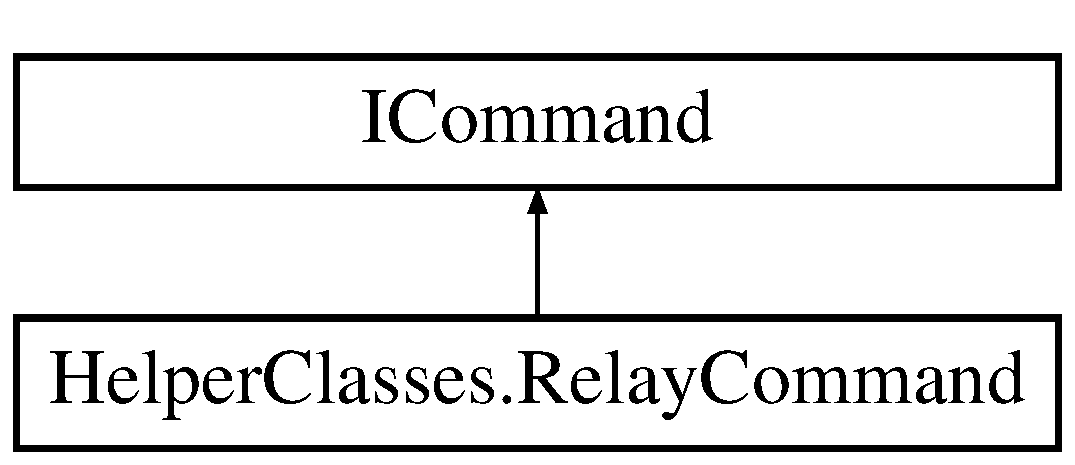
\includegraphics[height=2.000000cm]{class_helper_classes_1_1_relay_command}
\end{center}
\end{figure}
\subsection*{Public Member Functions}
\begin{DoxyCompactItemize}
\item 
\hyperlink{class_helper_classes_1_1_relay_command_adaa15c8188e458580150467e65570ae3}{Relay\+Command} (Action execute)
\begin{DoxyCompactList}\small\item\em Creates a new command that can always execute. \end{DoxyCompactList}\item 
\hyperlink{class_helper_classes_1_1_relay_command_af502adcf702c1b82d7d152367ffd1841}{Relay\+Command} (Action execute, Func$<$ bool $>$ can\+Execute)
\begin{DoxyCompactList}\small\item\em Creates a new command. \end{DoxyCompactList}\item 
bool \hyperlink{class_helper_classes_1_1_relay_command_a1e2d080059a2f0f7cd455af612d77bbe}{Can\+Execute} (object parameter)
\begin{DoxyCompactList}\small\item\em Determines whether this \hyperlink{class_helper_classes_1_1_relay_command}{Relay\+Command} can execute in its current state. \end{DoxyCompactList}\item 
void \hyperlink{class_helper_classes_1_1_relay_command_aea3b6adf254deec1cb6ef1652070444b}{Execute} (object parameter)
\begin{DoxyCompactList}\small\item\em Executes the \hyperlink{class_helper_classes_1_1_relay_command}{Relay\+Command} on the current command target. \end{DoxyCompactList}\item 
void \hyperlink{class_helper_classes_1_1_relay_command_a14af980403ef90c4ee57f1395988fa8e}{Raise\+Can\+Execute\+Changed} ()
\begin{DoxyCompactList}\small\item\em Method used to raise the \hyperlink{class_helper_classes_1_1_relay_command_a2e0f01d199cf4ba351ba10aa7c9c85c4}{Can\+Execute\+Changed} event to indicate that the return value of the \hyperlink{class_helper_classes_1_1_relay_command_a1e2d080059a2f0f7cd455af612d77bbe}{Can\+Execute} method has changed. \end{DoxyCompactList}\end{DoxyCompactItemize}
\subsection*{Events}
\begin{DoxyCompactItemize}
\item 
Event\+Handler \hyperlink{class_helper_classes_1_1_relay_command_a2e0f01d199cf4ba351ba10aa7c9c85c4}{Can\+Execute\+Changed}
\begin{DoxyCompactList}\small\item\em Raised when Raise\+Can\+Execute\+Changed is called. \end{DoxyCompactList}\end{DoxyCompactItemize}


\subsection{Detailed Description}
A command whose sole purpose is to relay its functionality to other objects by invoking delegates. The default return value for the Can\+Execute method is \textquotesingle{}true\textquotesingle{}. \hyperlink{class_helper_classes_1_1_relay_command_a14af980403ef90c4ee57f1395988fa8e}{Raise\+Can\+Execute\+Changed} needs to be called whenever \hyperlink{class_helper_classes_1_1_relay_command_a1e2d080059a2f0f7cd455af612d77bbe}{Can\+Execute} is expected to return a different value. 



\subsection{Constructor \& Destructor Documentation}
\hypertarget{class_helper_classes_1_1_relay_command_adaa15c8188e458580150467e65570ae3}{}\index{Helper\+Classes\+::\+Relay\+Command@{Helper\+Classes\+::\+Relay\+Command}!Relay\+Command@{Relay\+Command}}
\index{Relay\+Command@{Relay\+Command}!Helper\+Classes\+::\+Relay\+Command@{Helper\+Classes\+::\+Relay\+Command}}
\subsubsection[{Relay\+Command}]{\setlength{\rightskip}{0pt plus 5cm}Helper\+Classes.\+Relay\+Command.\+Relay\+Command (
\begin{DoxyParamCaption}
\item[{Action}]{execute}
\end{DoxyParamCaption}
)}\label{class_helper_classes_1_1_relay_command_adaa15c8188e458580150467e65570ae3}


Creates a new command that can always execute. 


\begin{DoxyParams}{Parameters}
{\em execute} & The execution logic.\\
\hline
\end{DoxyParams}
\hypertarget{class_helper_classes_1_1_relay_command_af502adcf702c1b82d7d152367ffd1841}{}\index{Helper\+Classes\+::\+Relay\+Command@{Helper\+Classes\+::\+Relay\+Command}!Relay\+Command@{Relay\+Command}}
\index{Relay\+Command@{Relay\+Command}!Helper\+Classes\+::\+Relay\+Command@{Helper\+Classes\+::\+Relay\+Command}}
\subsubsection[{Relay\+Command}]{\setlength{\rightskip}{0pt plus 5cm}Helper\+Classes.\+Relay\+Command.\+Relay\+Command (
\begin{DoxyParamCaption}
\item[{Action}]{execute, }
\item[{Func$<$ bool $>$}]{can\+Execute}
\end{DoxyParamCaption}
)}\label{class_helper_classes_1_1_relay_command_af502adcf702c1b82d7d152367ffd1841}


Creates a new command. 


\begin{DoxyParams}{Parameters}
{\em execute} & The execution logic.\\
\hline
{\em can\+Execute} & The execution status logic.\\
\hline
\end{DoxyParams}


\subsection{Member Function Documentation}
\hypertarget{class_helper_classes_1_1_relay_command_a1e2d080059a2f0f7cd455af612d77bbe}{}\index{Helper\+Classes\+::\+Relay\+Command@{Helper\+Classes\+::\+Relay\+Command}!Can\+Execute@{Can\+Execute}}
\index{Can\+Execute@{Can\+Execute}!Helper\+Classes\+::\+Relay\+Command@{Helper\+Classes\+::\+Relay\+Command}}
\subsubsection[{Can\+Execute}]{\setlength{\rightskip}{0pt plus 5cm}bool Helper\+Classes.\+Relay\+Command.\+Can\+Execute (
\begin{DoxyParamCaption}
\item[{object}]{parameter}
\end{DoxyParamCaption}
)}\label{class_helper_classes_1_1_relay_command_a1e2d080059a2f0f7cd455af612d77bbe}


Determines whether this \hyperlink{class_helper_classes_1_1_relay_command}{Relay\+Command} can execute in its current state. 


\begin{DoxyParams}{Parameters}
{\em parameter} & Data used by the command. If the command does not require data to be passed, this object can be set to null. \\
\hline
\end{DoxyParams}
\begin{DoxyReturn}{Returns}
true if this command can be executed; otherwise, false.
\end{DoxyReturn}
\hypertarget{class_helper_classes_1_1_relay_command_aea3b6adf254deec1cb6ef1652070444b}{}\index{Helper\+Classes\+::\+Relay\+Command@{Helper\+Classes\+::\+Relay\+Command}!Execute@{Execute}}
\index{Execute@{Execute}!Helper\+Classes\+::\+Relay\+Command@{Helper\+Classes\+::\+Relay\+Command}}
\subsubsection[{Execute}]{\setlength{\rightskip}{0pt plus 5cm}void Helper\+Classes.\+Relay\+Command.\+Execute (
\begin{DoxyParamCaption}
\item[{object}]{parameter}
\end{DoxyParamCaption}
)}\label{class_helper_classes_1_1_relay_command_aea3b6adf254deec1cb6ef1652070444b}


Executes the \hyperlink{class_helper_classes_1_1_relay_command}{Relay\+Command} on the current command target. 


\begin{DoxyParams}{Parameters}
{\em parameter} & Data used by the command. If the command does not require data to be passed, this object can be set to null. \\
\hline
\end{DoxyParams}
\hypertarget{class_helper_classes_1_1_relay_command_a14af980403ef90c4ee57f1395988fa8e}{}\index{Helper\+Classes\+::\+Relay\+Command@{Helper\+Classes\+::\+Relay\+Command}!Raise\+Can\+Execute\+Changed@{Raise\+Can\+Execute\+Changed}}
\index{Raise\+Can\+Execute\+Changed@{Raise\+Can\+Execute\+Changed}!Helper\+Classes\+::\+Relay\+Command@{Helper\+Classes\+::\+Relay\+Command}}
\subsubsection[{Raise\+Can\+Execute\+Changed}]{\setlength{\rightskip}{0pt plus 5cm}void Helper\+Classes.\+Relay\+Command.\+Raise\+Can\+Execute\+Changed (
\begin{DoxyParamCaption}
{}
\end{DoxyParamCaption}
)}\label{class_helper_classes_1_1_relay_command_a14af980403ef90c4ee57f1395988fa8e}


Method used to raise the \hyperlink{class_helper_classes_1_1_relay_command_a2e0f01d199cf4ba351ba10aa7c9c85c4}{Can\+Execute\+Changed} event to indicate that the return value of the \hyperlink{class_helper_classes_1_1_relay_command_a1e2d080059a2f0f7cd455af612d77bbe}{Can\+Execute} method has changed. 



\subsection{Event Documentation}
\hypertarget{class_helper_classes_1_1_relay_command_a2e0f01d199cf4ba351ba10aa7c9c85c4}{}\index{Helper\+Classes\+::\+Relay\+Command@{Helper\+Classes\+::\+Relay\+Command}!Can\+Execute\+Changed@{Can\+Execute\+Changed}}
\index{Can\+Execute\+Changed@{Can\+Execute\+Changed}!Helper\+Classes\+::\+Relay\+Command@{Helper\+Classes\+::\+Relay\+Command}}
\subsubsection[{Can\+Execute\+Changed}]{\setlength{\rightskip}{0pt plus 5cm}Event\+Handler Helper\+Classes.\+Relay\+Command.\+Can\+Execute\+Changed}\label{class_helper_classes_1_1_relay_command_a2e0f01d199cf4ba351ba10aa7c9c85c4}


Raised when Raise\+Can\+Execute\+Changed is called. 



The documentation for this class was generated from the following file\+:\begin{DoxyCompactItemize}
\item 
d\+:/\+Dokumenter/\+Visual Studio 2013/\+Projects/2. Semester/\+Kanban\+Board/\+Kanban\+Board/\+Relay\+Command/Relay\+Command.\+cs\end{DoxyCompactItemize}

%--- End generated contents ---

% Index
\backmatter
\newpage
\phantomsection
\clearemptydoublepage
\addcontentsline{toc}{chapter}{Index}
\printindex

\end{document}
